\chapter{Design}
\label{chap:fejezet8}

A Design-t összesen 3 CSS fájllal oldottam meg. Ezek a fájlok a rendelo/static/Css mappában találhatók:

\begin{itemize}
	\item style.css: Az oldalak kinézetét írtam meg benne színek nélkül.
	\item colors\_light.css: Az alkalmazás világos módjának a színbeállításait írtam meg benne.
	\item colors\_dark.css: Az alkalmazás világos módjának a színbeállításait írtam meg benne.
\end{itemize}

\begin{figure}[H]
	\caption{A "base.html" kinézete, és a navbar világos módban}
	\label{fig:lightmode}
	\centering
	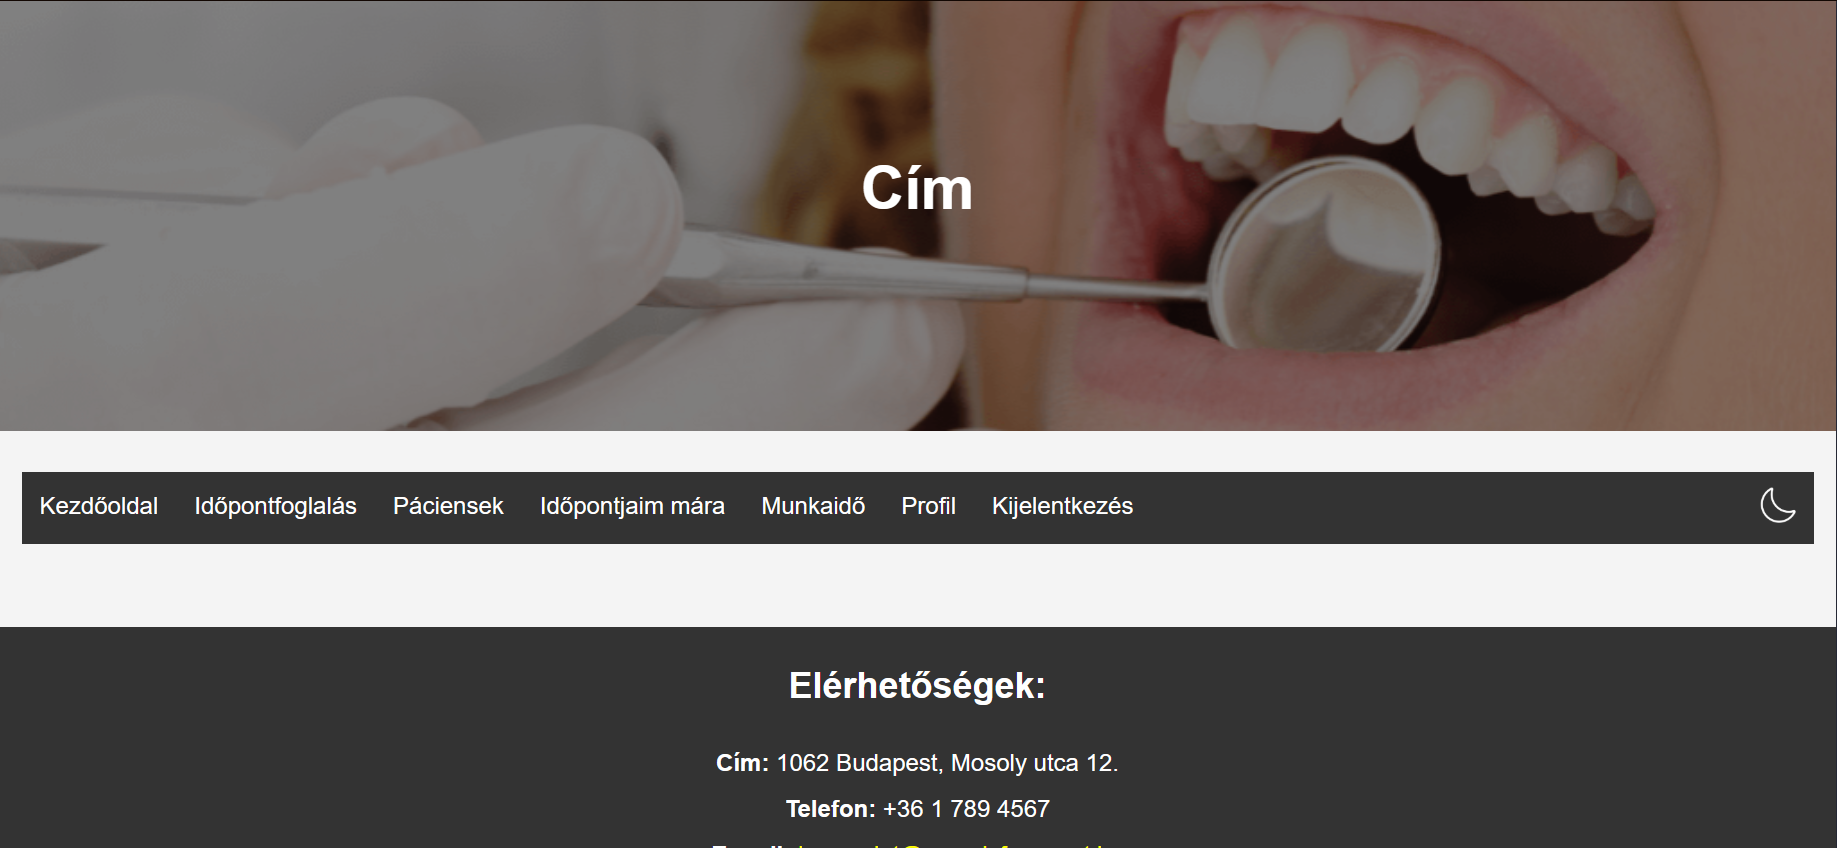
\includegraphics[width=1.0\textwidth]{base_page_light.png}
\end{figure}

A 8.1. ábrán világos módban megtekinthető a "base.html". Ahogy korábban már írtam, ebből származik az összes többi oldal, így mindegyik ezt a designt követi. Sötét módba a navigációs sáv jobb oldalán lévő "hold" ikonnal léphetünk.

\begin{figure}[H]
	\caption{A "base.html" kinézete, és a navbar sötét módban}
	\label{fig:darkmode}
	\centering
	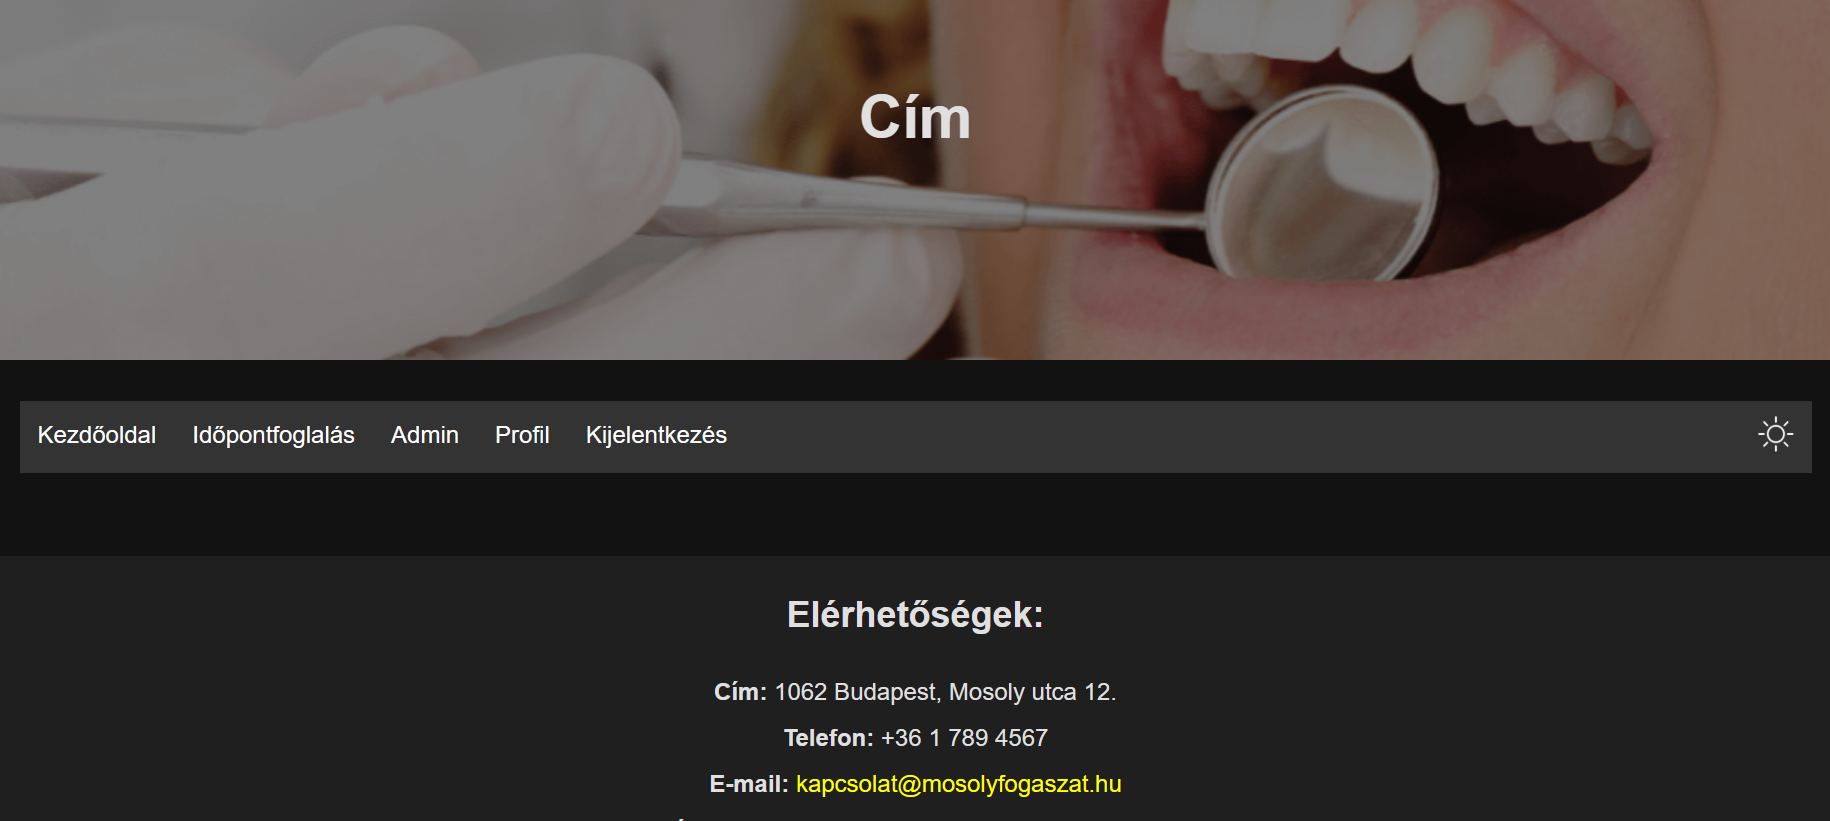
\includegraphics[width=1.0\textwidth]{base_page_dark.png}
\end{figure}

Ezt a "base.html" fájlban megírt JS kód hajtja végre:

\begin{lstlisting}[caption={A színösszeállítások között váltó JS kód},label={lst:stringstartswith2}, language={HTML}]
	<script>
	function toggleColorScheme() {
		const currentScheme = document.getElementById('color-scheme').getAttribute('href');
		const newScheme = currentScheme.includes('colors_light.css') ? 'colors_dark.css' : 'colors_light.css';
		document.getElementById('color-scheme').setAttribute('href', `` + newScheme);
		localStorage.setItem('color-scheme', newScheme);
		updateIcon(newScheme);
	}
	
	function updateIcon(scheme) {
		const icon = document.getElementById('color-scheme-icon');
		if (scheme.includes('colors_light.css')) {
			icon.src = '';
			icon.alt = 'Sotet mod';
		} else {
			icon.src = '';
			icon.alt = 'Vilagos mod';
		}
	}
	
	document.addEventListener('DOMContentLoaded', function() {
		const savedScheme = localStorage.getItem('color-scheme') || 'colors_light.css';
		document.getElementById('color-scheme').setAttribute('href', `` + savedScheme);
		updateIcon(savedScheme);
	});
	</script>
	
\end{lstlisting}

Alapértelmezetten a világos mód Css fájlját improtálja, viszont ha kattintunk a "hold" ikonra, akkor átírja az importot a sötét mód Css fájljának az importjára, majd utána átváltja "napra" az ikont, amire kattintottunk jelezve ezzel, hogy az a világos módba vezet. A design megírásához sima Css-t használtam.

